\chapter{Introduction}
\label{Introduction}
\thispagestyle{fancy}

\section{Présentation du produit}
\label{Introduction:Présentation du produit}
On présente ici de manière succincte l'architecture Hardware du robot Pepper afin de se familiariser avec les différents éléments du système que nous serons susceptible de rencontrer durant la mise en œuvre de ce projet.  

\subsection{Les actionneurs}
\label{Introduction:Présentation du produit:Les actionneurs}
\subsubsection{Les moteurs}
\label{Introduction:Présentation du produit:Les actionneurs: Les moteurs}
Le robot Pepper est constitué de 20 moteurs dont il est possible de contrôler la position et la rigidité. \ref*{fig:Répartition des actionneurs de Pepper}
\begin{description}
	\item [Tête:] 2 moteurs pour les mouvements de lacet (HeadYaw) et de tangage (HeadPitch)
	\item [Bras:] 4 moteurs par bras, répartis de la manière suivante: 
	\begin{description}
		\item [Épaule:] 2 moteurs pour les mouvements de tangage (ShoulderPitch) et de roulis du bras (ShoulderRoll).
		\item [Coude:] 2 moteurs pour les mouvements de lacet(ElbowRoll) et de lacet (ElbowYaw) de l'avant-bras.
	\end{description}
	\item [Main:] 1 moteur pour le mouvement de lacet du poignet (WristYaw) et 1 pour le mouvement d'ouverture et de fermeture de la main (Hand).
	\item [Hanche:] 2 moteurs pour le mouvement de roulis (HipRoll) et de tangage (HipPitch) du buste.
	\item [Genoux:] 1 moteur pour le mouvement de tangage (KneePitch) du haut du corps.
	\item [Roues:] 3 moteurs pour les mouvements en rotation de chacune des 3 roues omnidirectionnelles (WheelB, WheelFR et WheelFL).
\end{description}

\begin{figure}[h]
	\centering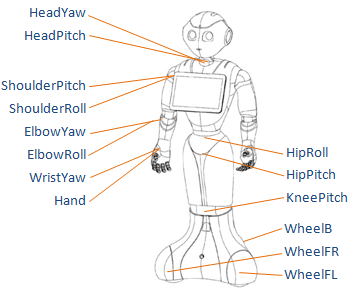
\includegraphics[height=7cm]{images/pepper_motors.png}
	\caption{Répartition des actionneurs de Pepper}
	\label{fig:Répartition des actionneurs de Pepper}
\end{figure}

\subsubsection{Les Leds}
\label{Introduction:Présentation du produit:Les actionneurs: Les leds}
Les leds placés sur les épaules de Pepper et autour de ces yeux permettent d'obtenir un certain nombre d'informations sur son état.

\subsection{Les senseurs}
\label{Introduction:Présentation du produit:Les senseurs}
Pepper comporte également une multitude de capteurs. Certains d'entre eux sont utilisés afin de s'assurer du bon comportement des parties électroniques et mécaniques du robot, ou pour réaliser du contrôle-commande. D'autres senseurs sont en revanche intégrés au robot pour que l'utilisateur puisse interagir avec. \ref{tab: Les différents capteurs de Pepper}

\begin{table}[h]
\begin{tabular}{ | p{3cm} | p{4cm} | p{7cm} | }
\hline
Senseur & position & description \\
\hline
Capteurs liés au actionneurs & sur les moteurs & Chaque moteur du robot est lié à 3 senseurs donnant des informations sur la valeur du courant délivrée au moteur (A), la température du moteur (C) et la position du moteur. \\
\hline
Senseurs tactiles & 1 sur chaque main, 1 sur la tête & Permet à l'utilisateur d'interagir avec le robot par le toucher.	\\	
\hline 
Les boutons & 1 sur le buste, 3 bumpers sur la base du robot & Les bumpers permettent au robot de détecter si il rencontre un obstacle à proximité directe. Le bouton du buste permet quant à lui de modifier le mode dans lequel est le robot (autonome, veille). \\
\hline 
Centrale inertielle & 1 dans le buste, 1 dans la base & Informe sur la position et l'orientation du robot, ainsi que les données qui en découlent (vitesse, accélération). \\
\hline
Sonars & 2 sonars à l'avant et l'arrière de la base & Permet de détecter la présence d'un objet situé à partir de 65 cm du robot. \\
\hline 
Capteurs batterie & Au niveau de la batterie & Renseigne sur le courant et la tension délivré, le pourcentage de charge et la température. \\
\hline
Capteurs infra-rouges & 2 sur la base &  Permet de détecter la présence d'un objet situé entre à et 50 cm du robot. \\
\hline
Lasers & 6 lasers sur la base du robot & Permet de détecter la présence d'un objet \\
\hline 
\end{tabular}
\caption[Les différents capteurs de Pepper]{Les différents capteurs de l'architecture sensorielle de Pepper}
\label {tab: Les différents capteurs de Pepper}
\end{table}


\section{Expression du besoin}
\label{Introduction:Expression du besoin}
L'extension du marché visée par Aldebaran pour Pepper s'accompagne d'une montée en puissance de la production. Afin de la guider, des outils de vérification des produits en fin de ligne de production sont mis en place. Parmi eux, on retrouve le "Filtering Test"\ref{tab: Déroulement d'un Filtering test} qui consiste à réaliser une série de tests durant six heures. Il vise notamment à stresser l'ensemble des parties mécaniques du robot afin de faire ressortir d'éventuelles erreurs. Si une anomalie survient lors du déroulement du test, les différentes données relatives à l'état des systèmes mécaniques et électroniques du robot sont enregistrées dans un fichier journal (e.g. température des fusibles, valeur des accéléromètres, etc.). Afin d'identifier les causes de l'apparition de problèmes sur Pepper, un certain nombre d'hypothèses sont émises à partir de l'étude des données en sortie du système. 

% Mettre à jour le déroulement du test à partir du code de Meigui et des explications de Thomas
\begin{table}[h]
	\begin{tabular}{ | p {4cm} | p {2.5cm} | p {2.5cm} |  p {4cm} |}
		\hline 
		\multicolumn{4}{| l |}{5 étapes successives sur 6 heures de test}\\
		\hline
		Activité & Durée (en minutes) & Temps cumulé (en minutes)  & Description\\
		\hline
		\multicolumn{4}{| l |}{Test 1 : succession de divers actions effectué 40 fois durant les 10 heures }\\
		\hline
		Intro, Danse, Outro & 6 à 7  & 6 à 7 & Réalisation des mouvements d'introduction et d'outro\\
		\hline 
		Cycles de WakeUp, Rest & 3 à 4  & 10  & Passage successif en mode autonome et veille\\
		\hline 
		Faux dialogues & 2  & 12 &  Réalisation des mouvements effectués lors de dialogues\\
		\hline 
		Rest & 3  & 15 & Réalisation des mouvements lors du passage en mode Rest\\
		\hline
		\multicolumn{4}{| l |}{Test 12: enchainement de 8 danses répété 5 fois durant les dix heures} \\
		\hline
	\end{tabular}
	\caption[Déroulement d'un Filtering test]{Déroulement d'un Filtering test}
	\label {tab: Déroulement d'un Filtering test}
\end{table}
 
\subsection{Hiérarchisation des erreurs}
\label{Introduction:Expression du besoin:Hiérarchisation des erreurs}
Afin de gérer au mieux les anomalies, celles-ci sont hiérarchisées en deux catégories.
\begin{description}
	\item [Error name] Il s'agit de l'erreur visible, c'est à dire de la conséquence liée à une anomalie hardware ou software. Cela peut correspondre par exemple à la chute du robot. 
	\item [root cause] Il s'agit de l'anomalie en elle même, c'est à dire de la cause ayant entraîné l'apparition d'une "error name". Si l' "error name" est la chute d'un robot, la "root cause" peut par exemple correspondre à la détérioration d'un engrenage de la hanche.   
\end{description} 

En suivant la logique exprimée par ces définitions, une "error name" sera constituée d'une ou plusieurs "root cause". 

\begin{forest}
	for tree={
		draw,
		minimum height=2cm,
		anchor=north,
		align=center,
		child anchor=north
	},
	[{Chute du robot}, align=center, name=CR
		[{Engrenage cassé}, name=EC]
		[{Courant dans les\\fusibles trop élevés}]
		[{Erreur de la\\centrale inertielle}]
	]

	\node[anchor=west,align=left] 
	at ([xshift=-2cm]MS.west|-EC) {Level 2\\Root cause};
	\node[anchor=west,align=left] 
	at ([xshift=-2cm]MS.west|-CR) {Level 1\\Error name};
\end{forest}


\subsection{Exemple d'analyse d'un fichier}
\label{Introduction:Expression du besoin:Exemple d'analyse d'un fichier}
\begin{description}
	\item[Observation:] 
	\begin{itemize}
		\item Lors du déroulement du test, le robot tombe à t = 16972 secondes, soit lorsque le robot réalise une séquence de mouvements particulière appelée "Heat Behavior". Les valeurs retournées par l'accéléromètre selon l'axe $Z$ attestent de cette chute.
		\item On analyse alors les données liées aux systèmes mécaniques et électroniques du robot pouvant avoir une relation directe ou indirecte avec sa chute.  Lorsque l'on étudie la vitesse de rotation du moteur de la hanche, on remarque qu'aux environs de  t = 16970 secondes (c'est-à-dire 2 secondes avant la chute du robot), l'information fournie par le senseur ne suit plus la commande  envoyée au moteur.
		%Préviser à quel moment l'augmentation du courant arrive
		\item On remarque également une augmentation anormale du courant dans le moteur de l'articulation. 
	\end{itemize} 
	\item [Hypothèse émise:] Lors de l'exécution de l' animation "Heat Behavior", le robot est amené à réaliser des mouvements amples au niveau de sa hanche entrainant un certain stress sur cette partie mécanique. Lorsque l'engrenage de la hanche arrive près de sa butée mécanique, celui-ci ne parvient pas à atteindre sa position zéro.  Ce phénomène occasionne une augmentation du courant délivré dans le moteur de l'articulation ce qui entraine le passage en mode protégé du robot, désactivant sa rigidité.  Sans cette rigidité, le robot tombe ("error name"). Une étude plus poussée nous apprendra que la "root cause" du problème correspondait à une dent cassé sur l'engrenage de la hanche. 
\end{description}


\section{Solution proposée}
De part la quantité d'informations à analyser, cette tâche peut rapidement devenir rébarbative, d'où le souhait d'automatiser ce processus d'investigation. De part la variabilité des types de données, on ne peut réduire le nombre d'information à analyser en recherchant des caractéristiques communes (e.g. moyenne, écart type, etc.). On se propose donc d'utiliser des approches algorithmiques plus poussées via des méthodes d'apprentissages automatiques (plus connues sous le terme anglais de Machine Learning). La multiplicité des modèles composant l'apprentissage automatique nous permettra de répondre au mieux à la problématique.